\section{Problem}

When a scene is being scanned with a laser, time of flight camera, structured 
light sensor or other device capable of obtain a depth map of the scene,
 a set of 3D points is obtained per frame, its 3D coordinates 
are relative to the scanning device. It is necessary to move the captured points, 
according to the device movement or rotation in order to maintain geometrical properties of the captured scene,
 positioning the 3D points into a common coordinate system, conserving 
the original scene structure. This problem becomes trivial if we know the device position and orientation 
for each frame or if we have a set of matches (common points)  between each pair of successive 
frames. But this does not occur in practice and additional problems arise due 
to the noise and imperfections of capturing devices.


In general, when the sensor is collecting the 3D points from the scene, 
 it is necessary to move or rotate it in order to capture new objects and surfaces,
 adding more information to the reconstructed model. But in order to be 
able to infer the correct position of each new frame, it is necessary to have an overlapping area with a previous one. 
 
The overlapping areas of the different views of a scene must be correctly 
aligned when registering the points in a common coordinate system. 
Thus, with each new frame more information is added to the scene, 
getting closer to the desired result. 

\section{Mathematical Definition}

A point cloud is a set of 3D euclidean space points and the problem of aligning several point clouds 
in order to form a complete 3D model, where intersecting areas overlap perfectly, 
is known as registration. Assuming that all point clouds form part of a 3D global model and they can be 
 positioned  consistently accord to this model.

Let  ${\vec{a_i}},{\vec{b_i}} \in \mathbb{R}^3;i = 1,2,...,N$ be two sets of 3D euclidean space points.

We want to find $R,\vec{t}$ that minimizes the following expression:
$$
\sum\limits_{i=1}^N || R\vec{a_i} - \vec{b_i} - \vec{t} || \ ,
$$

\noindent where $R$ is a  $3\times3$ rotation matrix and $\vec{t} \in \mathbb{R}^3$ is a translation vector.


In the case that the two sets are identical, the previous expression will have a minimum at zero.

We are interested in applying this minimization scheme to real life data, specifically to consecutive 
point clouds (with very small rotation and translation), registering a global 3D model of 
a real scene. In order to align the point clouds, it is necessary to have an important overlapping 
area, which is equivalent to a very small rotation and translation of the sensor capturing the point clouds, 
this area will allow minimizing distances between pairs of points corresponding to the same real world position.


\begin{figure}[H]
\begin{subfigure}[b]{0.5\textwidth}

\includegraphics[scale=0.3]{images/two_clouds_1}
\caption{Point cloud A}
\end{subfigure}
\begin{subfigure}[b]{0.5\textwidth}
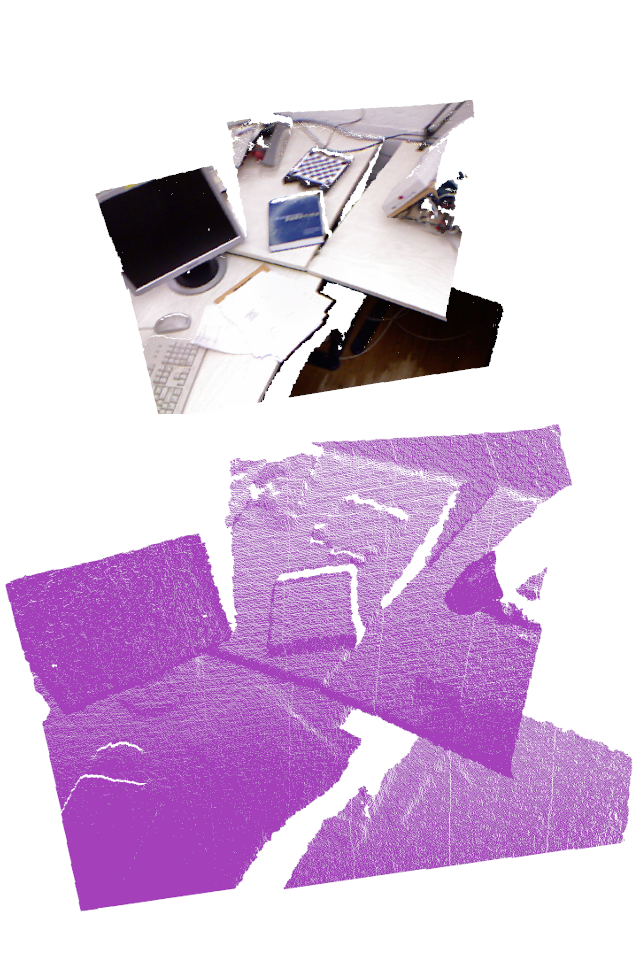
\includegraphics[scale=0.3]{images/two_clouds_2}
\caption{Point cloud B}
\end{subfigure}
\caption{Two point clouds corresponding to a real life scene. We want to find the correct rotation and translation to align both point clouds.}
\end{figure}

